\documentclass[conference]{IEEEtran}
\IEEEoverridecommandlockouts
% The preceding line is only needed to identify funding in the first footnote. If that is unneeded, please comment it out.

%\usepackage{cite}
\usepackage{amsmath,amssymb,amsfonts}
\usepackage{algorithmic}
\usepackage{graphicx}
\usepackage{textcomp}
\usepackage{xcolor}
\usepackage{comment}
\usepackage{amsfonts,graphicx,amsmath,amssymb,tikz}
\usepackage{parskip}

\usepackage{amsfonts}
\usepackage{multirow}
\usepackage{listings}
\usepackage[left=2cm, right=2cm, top=2cm]{geometry}
\usepackage{float}
\usepackage[sorting=none]{biblatex}
\usepackage{afterpage}
\usepackage{multirow}
\usepackage{textcomp}
\usepackage{gensymb}
\usepackage{amsmath}
\usepackage{graphicx}
\usepackage{subfigure}
\usepackage{enumitem}



\definecolor{codegreen}{rgb}{0,0.6,0}
\definecolor{codegray}{rgb}{0.5,0.5,0.5}
\definecolor{codepurple}{rgb}{0.58,0,0.82}
\definecolor{backcolour}{rgb}{0.95,0.95,0.92}
 
\lstdefinestyle{mystyle}{
    backgroundcolor=\color{backcolour},   
    commentstyle=\color{codegreen},
    keywordstyle=\color{magenta},
    numberstyle=\tiny\color{codegray},
    stringstyle=\color{codepurple},
    basicstyle=\ttfamily\footnotesize,
    breakatwhitespace=false,         
    breaklines=true,                 
    captionpos=b,                    
    keepspaces=true,                 
    numbers=left,                    
    numbersep=5pt,                  
    showspaces=false,                
    showstringspaces=false,
    showtabs=false,                  
    tabsize=2
}
\lstset{style=mystyle}


\usepackage{hyperref}
\hypersetup{ colorlinks, citecolor=blue, filecolor=black, linkcolor=blue, urlcolor=blue } 
\newcommand{\vecthree}[3]{\begin{pmatrix} #1 \\ #2 \\ #3 \end{pmatrix}}
\newcommand{\vecfour}[4]{\begin{pmatrix} #1 \\ #2 \\ #3 \\ #4\end{pmatrix}}
\newcommand{\mat}[1]{\boldsymbol { \mathsf{#1}} }

\DeclareMathOperator*{\argmax}{arg\,max}
\DeclareMathOperator*{\argmin}{arg\,min}
\newcommand{\norm}[1]{\lVert#1\rVert}
\newcommand{\R}{\mathbb{R}}

\definecolor{mycolor}{rgb}{0,0.6,0.5}


% Separate file for references
\addbibresource{references.bib}

\begin{document}

\title{Ray Tracing using Vulkan}

\author{\IEEEauthorblockN{Aiman Khan}
\IEEEauthorblockA{June 2023 \\
\textit{MSc Computer Game Engineering} \\
\textit{Computer Sciences, Newcastle University}\\
United Kingdom \\
c2055955@newcastle.ac.uk}
}

\maketitle

\begin{abstract}
    Ray tracing and rasterization are two fundamental techniques used in computer graphics for rendering. Rasterization operates by sequentially projecting each triangle onto a 2D screen, computing the pixels covered by the triangle, and using shader programs to determine the color of these pixels. Whereas ray tracing works by tracing rays from the camera's viewpoint, through each pixel of the image plane, and into the scene. While rasterization has been the dominant approach for many years due to its efficiency, ray tracing offers unparalleled visual fidelity and highly photorealistic renders without using complex techniques as used in rasterization to obtain similar effects. This research project demonstrates a ray tracing engine using Vulkan's ray tracing extension, and compares the render quality and computation performance metrics of ray traced images to rasterized images. By harnessing Vulkan's hardware acceleration capabilities, ray tracing can now achieve accelerated computation of ray-object intersections, enabling real-time rendering of complex scenes with advanced lighting effects, reflections, and global illumination, making it a compelling alternative to rasterization. The seamless integration of this ray tracing extension with existing Vulkan rendering pipelines provides flexibility in combining different rendering techniques in the same rendering engine. Moreover, Vulkan's cross-platform support ensures compatibility across various operating systems and hardware architectures, making it an appealing choice for developers. 
\end{abstract}

\begin{IEEEkeywords}
Ray Tracing Ray Casting, Rasterization, Vulkan, Vulkan's ray tracing extension, Hardware Acceleration, Real-time Rendering, Acceleration Structure, Shader Binding Table, Ray Tracing Pipeline
\end{IEEEkeywords}

\section{Introduction} \label{introduction}
Ray tracing has emerged as a powerful rendering technique in computer graphics, enabling the generation of highly realistic and visually stunning images. Traditional rendering approaches, such as rasterization, often struggle to accurately simulate the complex behavior of light, resulting in images that lack realism. In contrast, ray tracing mimics the physical behavior of light by tracing the path of individual rays through a virtual scene, calculating the interactions between rays and objects to determine pixel colors.

Ray tracing is a much better approach to rendering than rasterization because ray tracing accurately simulates light interactions, resulting in realistic shadows, reflections, and global illumination, while rasterization relies on approximations and additional techniques to achieve similar effects. The rasterization process takes a single triangle at a time, computes the pixels occupied by the triangle on a 2D screen and colors it using shader programs \cite{NVIDIA_raytracing_vs_rasterization}. The hardware currently processing a single triangle has no knowledge of the entire scene, and that is why to achieve effects like shadows, reflections, refraction, and global illumination, it requires additional workarounds in a rasterization pipeline.

\subsection{Ray Tracing Overview}
Ray tracing is a simulation for how light behaves in the real world. We see objects when photons coming from a light source bounce off that object into our eye. However when 3D rendering, we can not account for all rays coming from a light source, as some of then might not even hit the objects in our scene. To solve this problem, we reduce the rays coming from the light source to only include the rays that will hit the objects in our scene. Even with this limitation, most of the rays that bounce off the objects might not even reach the camera responsible for rendering. Therefore, for efficient rendering and to ensure there is no wasted computation, we cast rays from the camera's viewpoint through each pixel on the image plane, intersecting them with objects in the scene. Upon intersection, secondary rays can be generated, such as reflection and refraction rays, to model the effects of light bouncing off surfaces or passing through transparent materials \cite{Ray_Tracing_Gems}. This process of finding the hitpoint on the closest object as a ray leaves through the camera is known as \textit{ray casting}. 

Ray tracing is a computationally expensive process as it requires millions of ray object intersections per frame These rays are primary rays fired through each pixel and secondary and tertiary rays for shadow ray casting, reflection and refraction calculations. Furthermore, anti-aliasing techniques, which are crucial for producing smooth and visually appealing results, require casting multiple rays per pixel, further adding to the computational cost \cite{Ray_Tracing_Gems}. Therefore, real-time ray tracing was nearly impossible to achieve in the past. However, advancements in hardware technology and software algorithms have made real-time ray tracing possible now.

One of the the main challenges in real-time ray tracing is the computational complexity of tracing rays and evaluating their intersections with objects in the scene \cite{Realtime_Ray_Tracing_and_its_use_for_Interactive_Global_Illumination}. This process requires substantial computational resources, including high-performance processors and efficient data structures for accelerating ray-object intersections.

In recent years, the introduction of specialized hardware, such as dedicated ray tracing cores in GPUs, has greatly accelerated ray tracing performance. NVIDIA's Turing architecture, for example, introduced real-time ray tracing capabilities with dedicated hardware units called RT Cores \cite{NVIDIA_Turing_GPU_Architecture,Examination_RTX}. These dedicated units are specifically designed to accelerate ray tracing operations, making real-time ray tracing viable for applications like gaming and interactive graphics.

Furthermore, advancements in algorithms and techniques have played a crucial role in enabling real-time ray tracing. Improved spatial data structures, like bounding volume hierarchies (BVH), have enhanced ray-object intersection tests and scene traversal efficiency \cite{BVH_for_ray_tracing}. Additionally, techniques such as hierarchical culling and adaptive sampling have optimized ray tracing performance by reducing unnecessary computations and focusing resources on areas of the scene that require more accurate rendering \cite{Mattausch2015CHCRTCH}.

\begin{figure}[h]
    \centering
    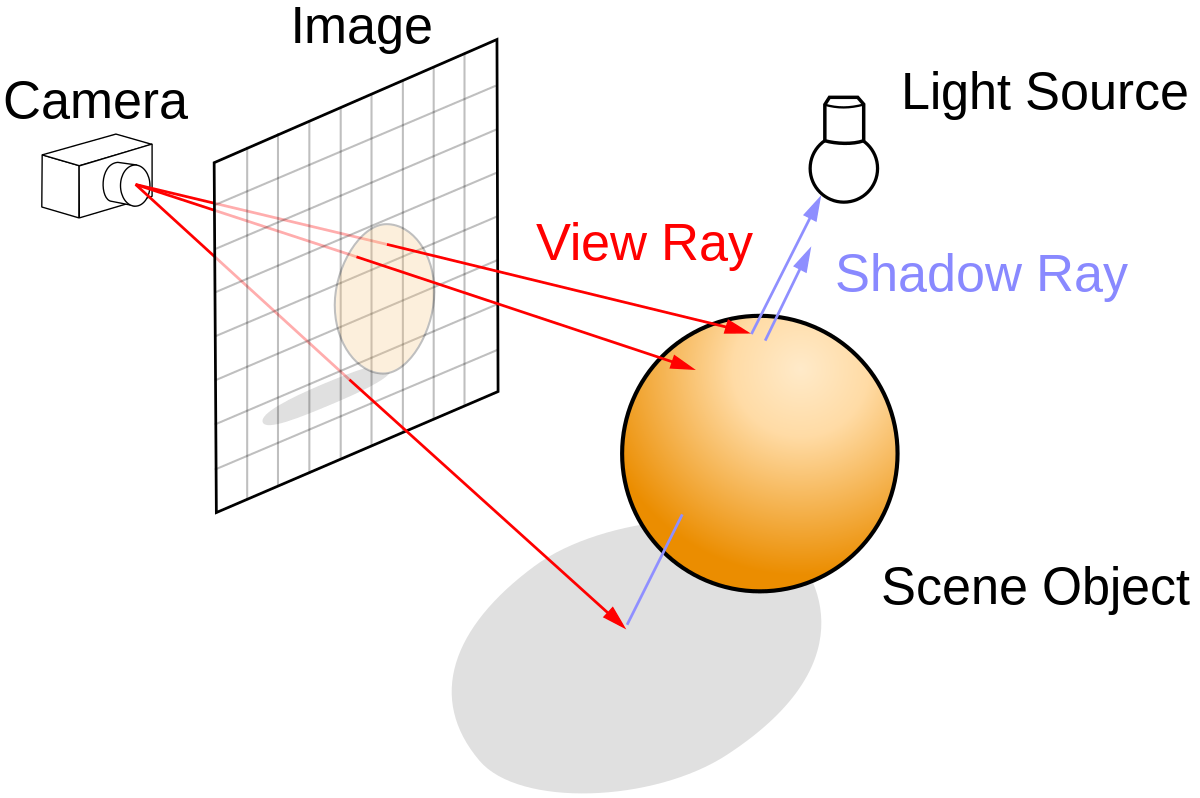
\includegraphics[scale=0.2]{figures/Ray_tracing_process.png}
    \caption{Ray Tracing Process \cite{NVIDIA_ray_tracing}}
    \label{ray_tracing_process}
\end{figure}

\begin{figure}[h]
    \centering
    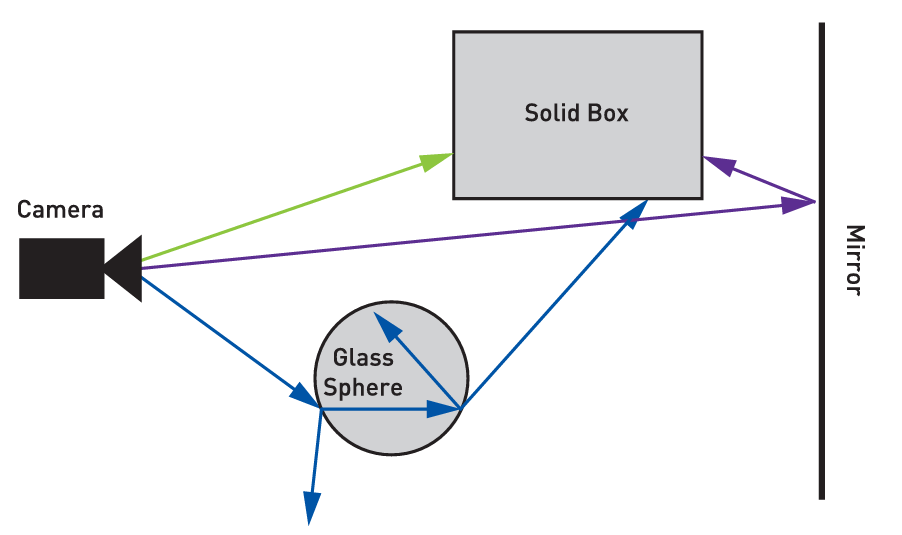
\includegraphics[scale=0.45]{figures/Ray_tracing_process_glass_mirror.png}
    \caption{Ray Tracing Process for Mirrors and Transparent Objects \cite{NVIDIA_ray_tracing}}
    \label{ray_tracing_process_glass_mirror}
\end{figure}

\subsection{Ray Tracing with Vulkan}
The Khronos Vulkan Ray Tracing Task Sub Group (TSG) published a ray tracing extension in 2020 that enables developers to leverage hardware-accelerated ray tracing capabilities \cite{KHR_Vulkan_Ray_Tracing}. Vulkan's ray tracing extension provides the following benefits, making it an appealing choice for rendering engines:

\begin{enumerate}
    \item Hardware Acceleration - Vulkan's ray tracing extension leverages specialized hardware, such as GPUs with dedicated ray tracing cores, to accelerate the ray tracing process. This hardware acceleration enables efficient computation of complex ray-object intersections and traversal of scenes, resulting in improved performance and faster rendering times thereby allowing real-time rendering \cite{KHR_Vulkan_Ray_Tracing}.
    \item Integration with Existing Rendering Pipelines - Vulkan's ray tracing extension seamlessly integrates with existing Vulkan rendering pipelines. This means that developers can combine ray tracing with other rendering techniques, such as rasterization or compute shaders, to achieve hybrid rendering approaches that combine the strengths of different algorithms. This flexibility enables the creation of visually stunning and computationally efficient graphics by leveraging the capabilities of both ray tracing and traditional rendering methods. Hence, the overall architecture adopted familiar elements and reused HLSL shaders, while introducing new features and implementation flexibility \cite{KHR_Vulkan_Ray_Tracing}.
    \item Developer Control and Flexibility: Vulkan's ray tracing extension provides developers with fine-grained control over the ray tracing pipeline. Developers can define custom shaders and algorithms, set up and manage acceleration structures efficiently, and optimize ray tracing operations to suit specific application requirements. This level of control empowers developers to tailor the ray tracing implementation to their specific needs, resulting in highly optimized and efficient rendering solutions \cite{KHR_Vulkan_Ray_Tracing}. 
    \item Cross-Platform Support: Vulkan is designed to be a cross-platform graphics API, making it compatible with a wide range of operating systems and hardware architectures. This cross-platform support ensures that applications utilizing Vulkan's ray tracing extension can run on various platforms, including Windows, Linux, and Android devices, without major modifications. This compatibility facilitates the widespread adoption and deployment of ray tracing techniques across multiple platforms \cite{KHR_Vulkan_Ray_Tracing}.
\end{enumerate}

\begin{comment}
\section{Related Work} \label{related-work}
Numerous studies have explored the advancements and applications of ray tracing in computer graphics. 

Recently, Vulkan's ray tracing extension has gained attention due to its potential for real-time ray tracing. By utilizing hardware-accelerated ray tracing, Vulkan allows for highly efficient rendering, making it suitable for applications that require interactive frame rates. A study by Laine et al. [2] demonstrated the benefits of using Vulkan's ray tracing extension, showcasing improved performance and visual quality compared to traditional ray tracing techniques.

Another noteworthy research effort by Jakob et al. [3] explored the integration of Vulkan's ray tracing extension with path tracing, a popular algorithm for simulating light transport in computer graphics. The combination of Vulkan's ray tracing capabilities with path tracing showed promising results in terms of rendering complex lighting effects and achieving high-quality visuals.

Furthermore, the work by Akenine-Möller et al. [4] investigated the utilization of Vulkan's ray tracing extension for real-time global illumination. By employing a combination of voxelization and ray tracing techniques, they demonstrated the potential of Vulkan in efficiently rendering dynamic scenes with realistic lighting.
\end{comment}
\section{Project Approach and Plan} \label{project-approach}
The aim of this project is to develop a ray tracing engine using Vulkan's ray tracing extension and compare the render quality and performance metrics with the results produced by a rasterization pipeline. The scene will be described a by .glTF scene file to ensure the comparison is performed on the same scene.

The current approach is to build a minimal ray tracing engine using the ray tracing extension of Vulkan and then work on to adding additional features like reflection, refraction, shadows, functionality to support more materials, and different types of lights etc into the rendering pipeline. to build a minimal ray tracing engine, following steps would be necessary \cite{NVIDIA_Vulkan_Ray_Tracing_Tutorial,Examination_RTX}: 

\begin{enumerate}
    \item Construct acceleration structures using the ray tracing extension API
    \item Create a ray tracing pipeline that includes the essential components of ray generation, closest hit, and miss shader programs. 
    \item Generate a shader table to bind the shader programs to the acceleration structures. 
    \item Create and execute command buffers on the established pipeline.
\end{enumerate}
\subsection{Acceleration Structure}
In order to achieve efficient ray tracing, it is crucial to organize the geometry into an acceleration structure (AS) that minimizes the number of ray-triangle intersection tests during rendering. This is typically implemented as a hierarchical structure in hardware, although the user is exposed to only two levels: a top-level acceleration structure (TLAS) and bottom-level acceleration structures (BLAS) \cite{NVIDIA_Vulkan_Ray_Tracing_Tutorial}. The TLAS serves as a reference to the BLAS and can include multiple instances, up to the maximum limit specified by VkPhysicalDeviceAccelerationStructurePropertiesKHR::maxInstanceCount. Each BLAS represents an individual 3D model within the scene, while the TLAS represents the entire scene constructed by positioning the referenced BLASes using transformation matrices (3-by-4 matrices) \cite{NVIDIA_Vulkan_Ray_Tracing_Tutorial}.

As shown in Figure \ref{acceleration_structure} The BLASes store the actual vertex data and are constructed from one or more vertex buffers, each with its own transformation matrix that is separate from the TLAS matrices \cite{NVIDIA_Vulkan_Ray_Tracing_Tutorial}. This allows for the storage of multiple positioned models within a single BLAS. %It is important to note that if an object is instantiated multiple times within the same BLAS, its geometry will be duplicated \cite{NVIDIA_Vulkan_Ray_Tracing_Tutorial}. This duplication can be advantageous for optimizing performance on static, non-instantiated components of the scene. As a general guideline, minimizing the number of BLASes tends to yield better performance \cite{NVIDIA_Vulkan_Ray_Tracing_Tutorial}.

The TLAS comprises object instances, each with its own transformation matrix and a reference to the corresponding BLAS. Initially, we begin with a single bottom-level AS and a top-level AS that instances it once using an identity transform \cite{NVIDIA_Vulkan_Ray_Tracing_Tutorial}.

\begin{figure}[h]
    \centering
    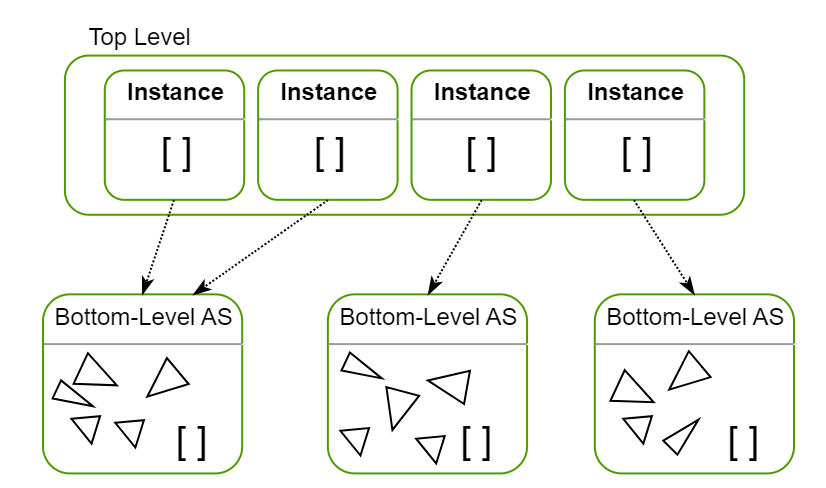
\includegraphics[scale=0.45]{figures/AccelerationStructure.png}
    \caption{Acceleration Structure \cite{NVIDIA_Vulkan_Ray_Tracing_Tutorial}}
    \label{acceleration_structure}
\end{figure}

\subsection{Ray Tracing Pipeline and the Shader Binding Table}
In the context of ray tracing, all shaders must be available for execution at any time during ray tracing, and the selection of shaders is done dynamically on the device at runtime \cite{NVIDIA_Vulkan_Ray_Tracing_Tutorial}. To enable this runtime shader selection, the creation of a Shader Binding Table (SBT) is essential. The SBT acts as a table of shader handles, similar to a C++ vtable \cite{NVIDIA_Vulkan_Ray_Tracing_Tutorial}. It needs to be constructed manually.

The entry point for ray tracing is the ray generation shader, which is invoked for each pixel. Typically, this shader initializes a ray starting from the camera's location, in a direction determined by evaluating the camera lens model at the pixel location. The ray generation shader then invokes traceRayEXT(), which shoots the ray into the scene. traceRayEXT, in turn, invokes subsequent shader types, allowing for communication of results using ray trace payloads \cite{NVIDIA_Vulkan_Ray_Tracing_Tutorial}.

The ray trace payloads are declared as rayPayloadEXT or rayPayloadInEXT variables, establishing a caller/callee relationship between shader stages. Each shader invocation creates a local copy of its declared rayPayloadEXT variables. When invoking another shader by calling traceRayEXT(), the caller can choose which payload to make visible to the callee shader as its rayPayloadInEXT variable (also known as the "incoming payload") \cite{NVIDIA_Vulkan_Ray_Tracing_Tutorial}.

Two important shader types to be utilized are the miss shader and the closest hit shader. The miss shader is executed when a ray does not intersect any geometry and can perform tasks such as sampling an environment map or returning a simple color through the ray payload \cite{NVIDIA_Vulkan_Ray_Tracing_Tutorial}. On the other hand, the closest hit shader is called when the ray hits the geometric instance closest to its starting point \cite{NVIDIA_Vulkan_Ray_Tracing_Tutorial}. This shader can handle lighting calculations and return the results through the ray payload. Multiple closest hit shaders can be used, similar to how a rasterization-based application has multiple pixel shaders for different objects \cite{NVIDIA_Vulkan_Ray_Tracing_Tutorial}.

\begin{comment}
    Optional shader types include the intersection shader, which allows intersecting user-defined geometry, and the any hit shader, which is executed on each potential intersection. The any hit shader is often useful for implementing efficient alpha-testing. It allows the ray traversal to continue without invoking traceRayEXT() again if the alpha test fails. In this example, any hit shaders will not be invoked since the opaque flag was specified during the acceleration structure construction.

\end{comment}
Figure \ref{pipeline} illustrates the structure of the Ray Tracing Pipeline. Initially, the pipeline includes only the three main shader programs: a single ray generation shader, a single miss shader, and a single hit group consisting solely of a closest hit shader. The GLSL shader programs are compiled into SPIR-V and linked together to form the ray tracing pipeline, which routes the intersection calculations to the appropriate hit shaders \cite{NVIDIA_Vulkan_Ray_Tracing_Tutorial}.

\begin{figure}[h]
    \centering
    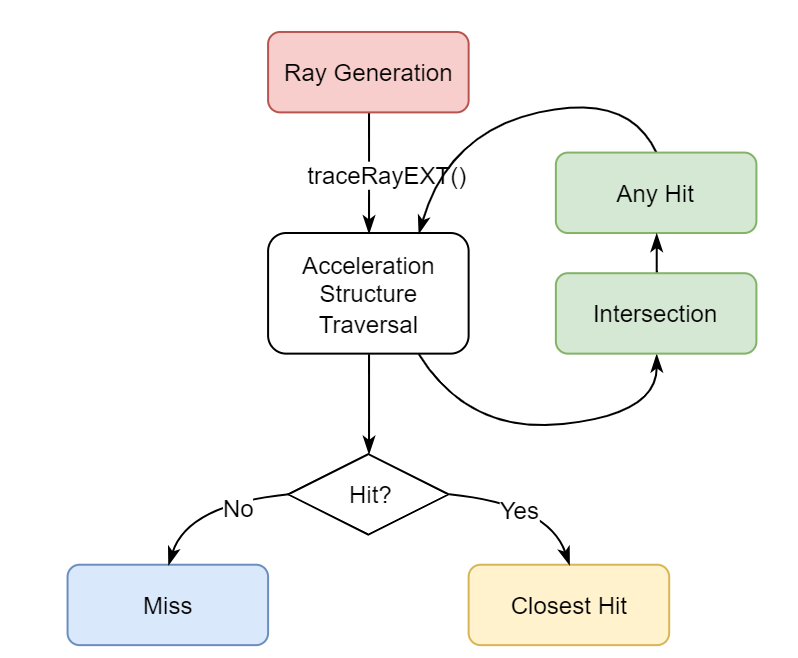
\includegraphics[scale=0.45]{figures/Ray_tracing_pipeline.png}
    \caption{Ray Tracing Pipeline \cite{NVIDIA_Vulkan_Ray_Tracing_Tutorial}}
    \label{pipeline}
\end{figure}

\subsection{Current Results}
Currently, a minimal ray tracing engine using Vulkan's ray tracing extension has been developed following tutorials from \cite{NVIDIA_Vulkan_Ray_Tracing_Tutorial} that incorporates basic lighting and a basic material. Figure \ref{fig:results} shows the results currently achieved and compares the rasterized and ray traced images. 
\begin{figure}%
    \centering
    \subfigure[\centering Rasterized Image]{{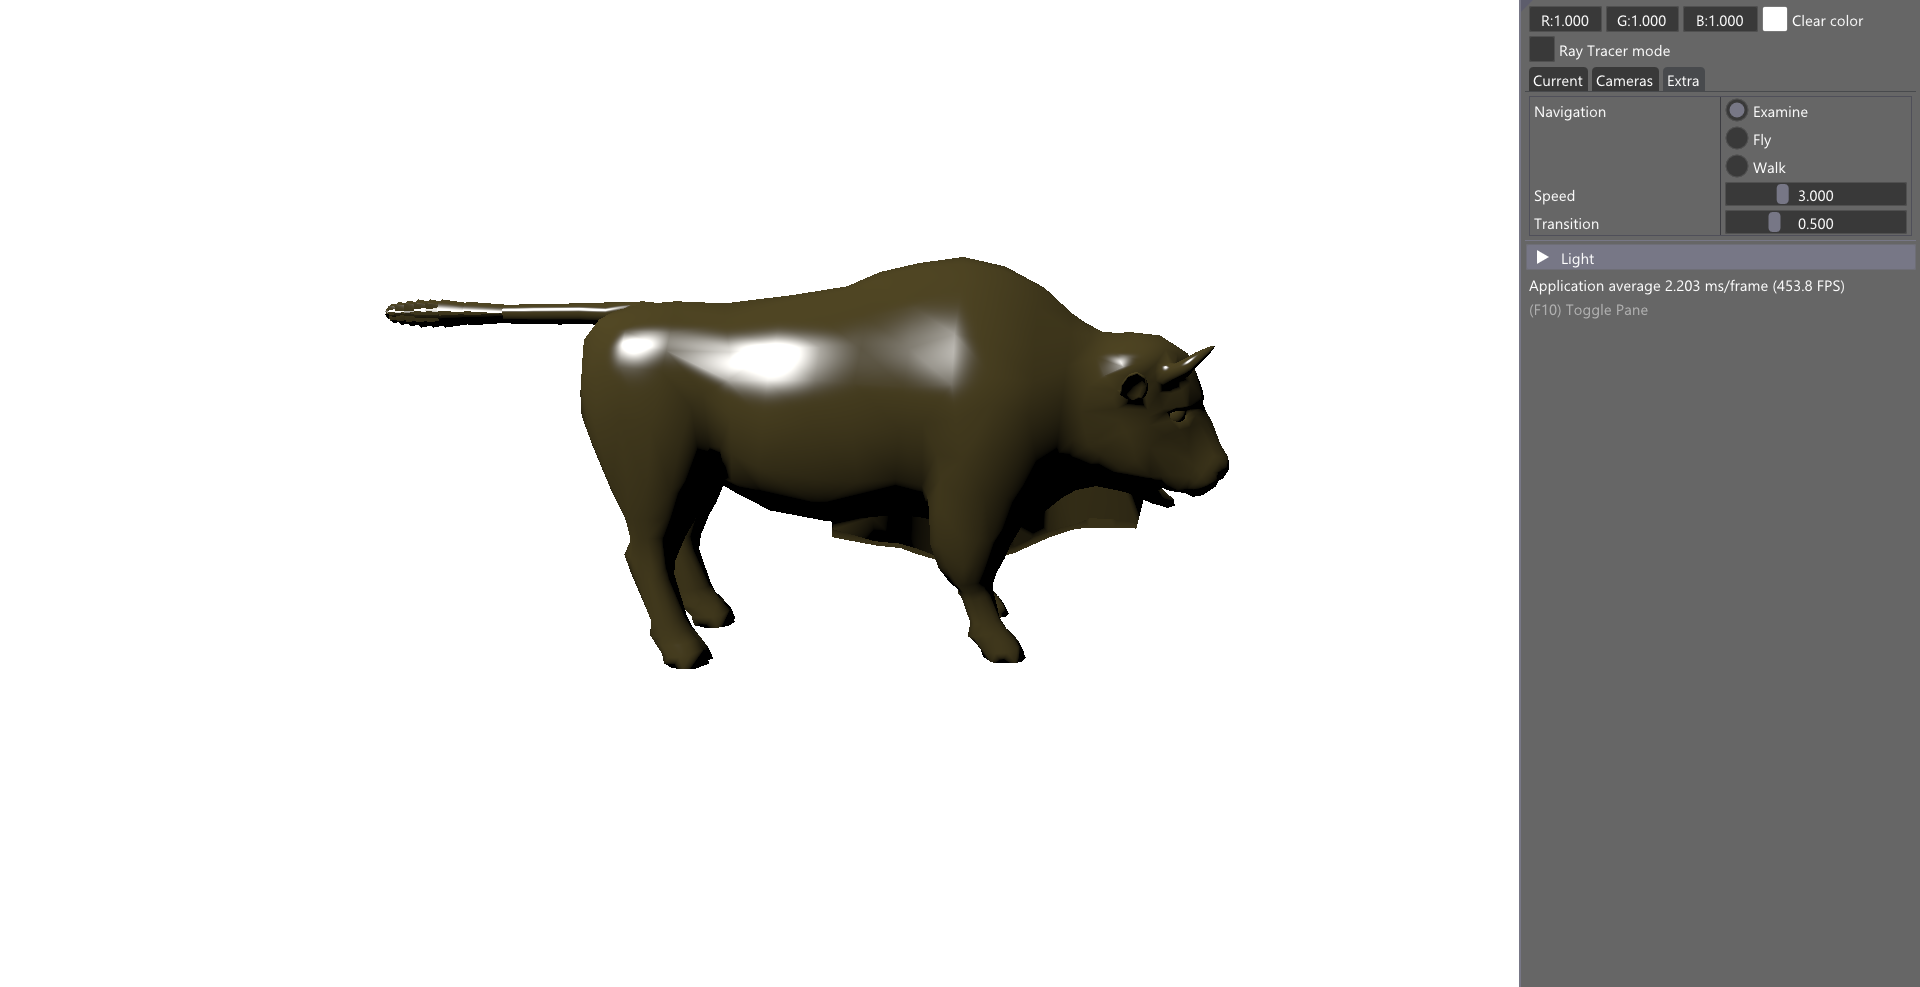
\includegraphics[scale=0.25]{figures/rasterized_image.png} }}%
    \qquad
    \subfigure[\centering Ray Traced Image]{{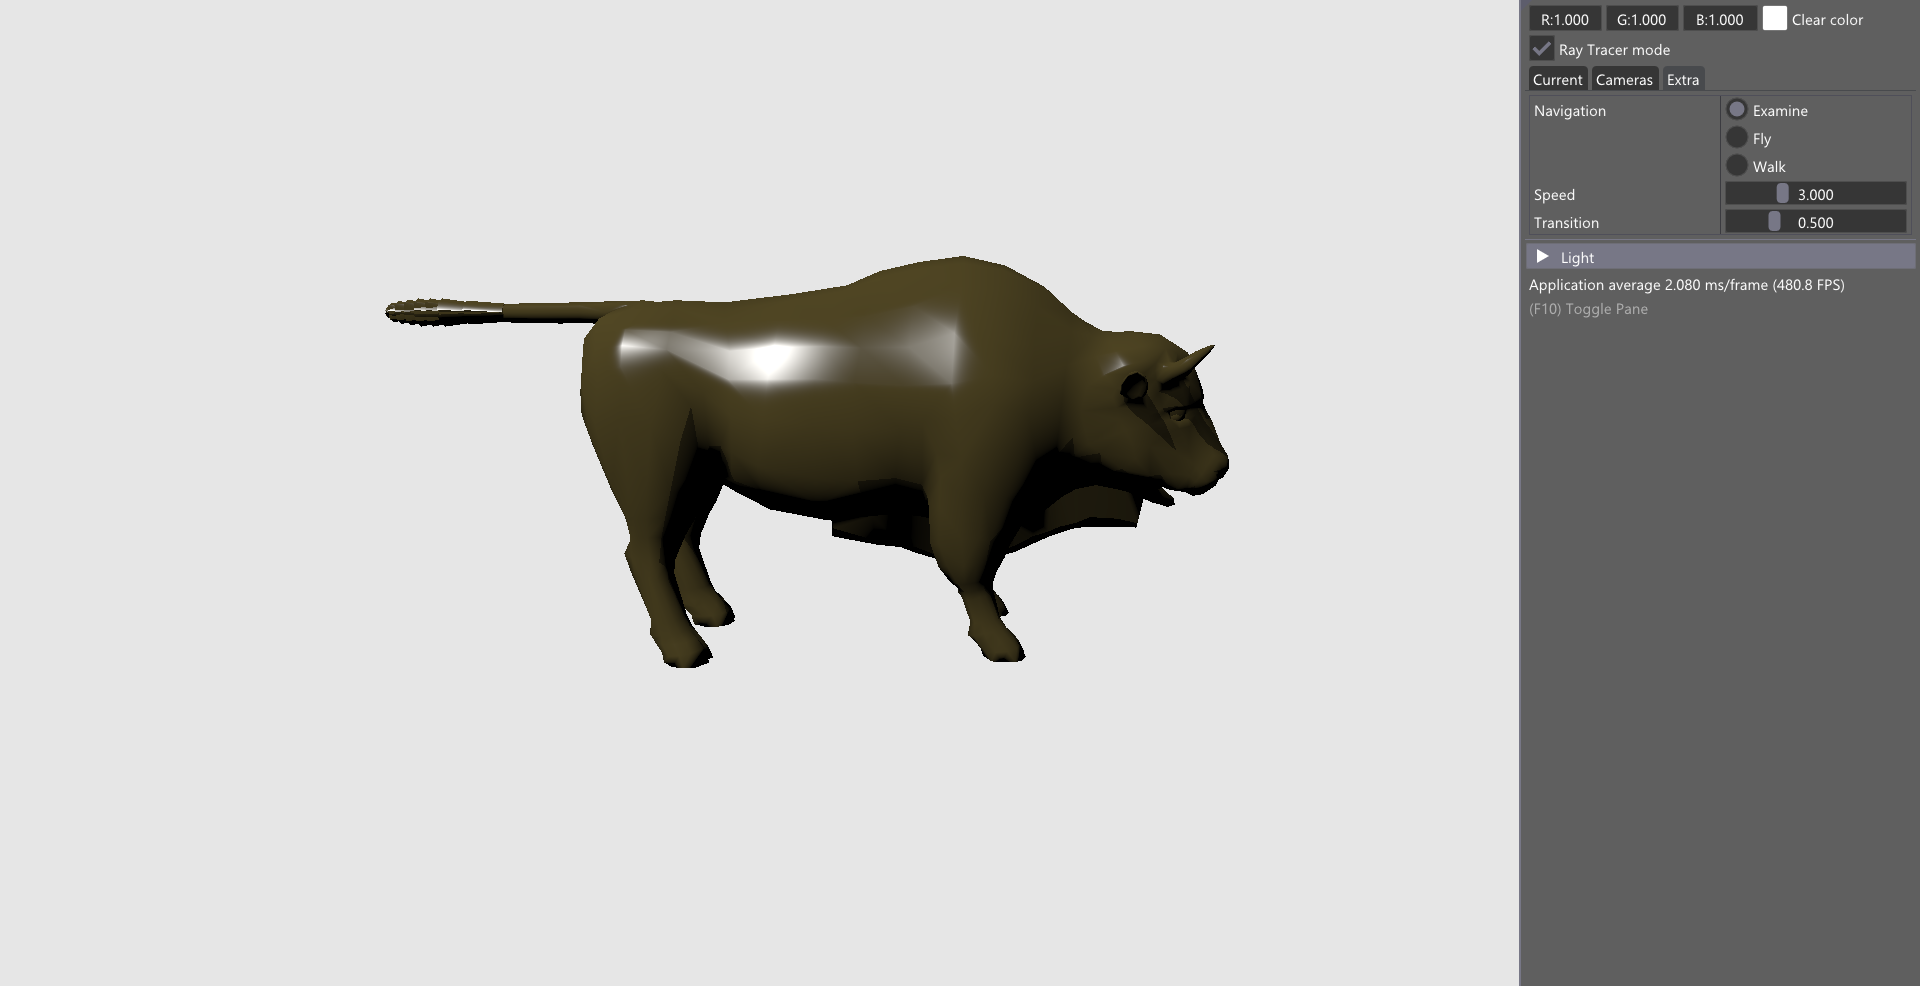
\includegraphics[scale=0.25]{figures/ray_traced_image.png} }}%
    \caption{Current Results}%
    \label{fig:results}%
\end{figure}
\printbibliography[heading=bibintoc,title={References}]
\end{document}
